\DeclareUnicodeCharacter{041B}{\CYRL}



\documentclass[11pt]{article}

    
    \usepackage{anyfontsize}
    \usepackage[breakable]{tcolorbox}
    \usepackage{parskip} % Stop auto-indenting (to mimic markdown behaviour)
    \usepackage[english,russian]{babel}
    \usepackage{graphicx}
    \usepackage{subcaption}

    % Basic figure setup, for now with no caption control since it's done
    % automatically by Pandoc (which extracts ![](path) syntax from Markdown).
    \usepackage{graphicx}
    % Maintain compatibility with old templates. Remove in nbconvert 6.0
    \let\Oldincludegraphics\includegraphics
    % Ensure that by default, figures have no caption (until we provide a
    % proper Figure object with a Caption API and a way to capture that
    % in the conversion process - todo).
    \usepackage{caption}

    \usepackage{float}
    \floatplacement{figure}{H} % forces figures to be placed at the correct location
    \usepackage{xcolor} % Allow colors to be defined
    \usepackage{enumerate} % Needed for markdown enumerations to work
    \usepackage{geometry} % Used to adjust the document margins
    \usepackage{amsmath} % Equations
    \usepackage{amssymb} % Equations
    \usepackage{textcomp} % defines textquotesingle
    % Hack from http://tex.stackexchange.com/a/47451/13684:
    \AtBeginDocument{%
        \def\PYZsq{\textquotesingle}% Upright quotes in Pygmentized code
    }
    \usepackage{upquote} % Upright quotes for verbatim code
    \usepackage{eurosym} % defines \euro

    \usepackage{iftex}
    \ifPDFTeX
        \usepackage[T1]{fontenc}
        \IfFileExists{alphabeta.sty}{
              \usepackage{alphabeta}
          }{
              \usepackage[mathletters]{ucs}
              \usepackage[utf8x]{inputenc}
          }
    \else
        \usepackage{fontspec}
        \usepackage{unicode-math}
    \fi

    \usepackage{fancyvrb} % verbatim replacement that allows latex
    \usepackage{grffile} % extends the file name processing of package graphics
                         % to support a larger range
    \makeatletter % fix for old versions of grffile with XeLaTeX
    \@ifpackagelater{grffile}{2019/11/01}
    {
      % Do nothing on new versions
    }
    {
      \def\Gread@@xetex#1{%
        \IfFileExists{"\Gin@base".bb}%
        {\Gread@eps{\Gin@base.bb}}%
        {\Gread@@xetex@aux#1}%
      }
    }
    \makeatother
    \usepackage[Export]{adjustbox} % Used to constrain images to a maximum size
    \adjustboxset{max size={0.9\linewidth}{0.9\paperheight}}

    % The hyperref package gives us a pdf with properly built
    % internal navigation ('pdf bookmarks' for the table of contents,
    % internal cross-reference links, web links for URLs, etc.)
    \usepackage{hyperref}
    % The default LaTeX title has an obnoxious amount of whitespace. By default,
    % titling removes some of it. It also provides customization options.
    \usepackage{titling}
    \usepackage{longtable} % longtable support required by pandoc >1.10
    \usepackage{booktabs}  % table support for pandoc > 1.12.2
    \usepackage{array}     % table support for pandoc >= 2.11.3
    \usepackage{calc}      % table minipage width calculation for pandoc >= 2.11.1
    \usepackage[inline]{enumitem} % IRkernel/repr support (it uses the enumerate* environment)
    \usepackage[normalem]{ulem} % ulem is needed to support strikethroughs (\sout)
                                % normalem makes italics be italics, not underlines
    \usepackage{mathrsfs}
    

    
    % Colors for the hyperref package
    \definecolor{urlcolor}{rgb}{0,.145,.698}
    \definecolor{linkcolor}{rgb}{.71,0.21,0.01}
    \definecolor{citecolor}{rgb}{.12,.54,.11}

    % ANSI colors
    \definecolor{ansi-black}{HTML}{3E424D}
    \definecolor{ansi-black-intense}{HTML}{282C36}
    \definecolor{ansi-red}{HTML}{E75C58}
    \definecolor{ansi-red-intense}{HTML}{B22B31}
    \definecolor{ansi-green}{HTML}{00A250}
    \definecolor{ansi-green-intense}{HTML}{007427}
    \definecolor{ansi-yellow}{HTML}{DDB62B}
    \definecolor{ansi-yellow-intense}{HTML}{B27D12}
    \definecolor{ansi-blue}{HTML}{208FFB}
    \definecolor{ansi-blue-intense}{HTML}{0065CA}
    \definecolor{ansi-magenta}{HTML}{D160C4}
    \definecolor{ansi-magenta-intense}{HTML}{A03196}
    \definecolor{ansi-cyan}{HTML}{60C6C8}
    \definecolor{ansi-cyan-intense}{HTML}{258F8F}
    \definecolor{ansi-white}{HTML}{C5C1B4}
    \definecolor{ansi-white-intense}{HTML}{A1A6B2}
    \definecolor{ansi-default-inverse-fg}{HTML}{FFFFFF}
    \definecolor{ansi-default-inverse-bg}{HTML}{000000}

    % common color for the border for error outputs.
    \definecolor{outerrorbackground}{HTML}{FFDFDF}

    % commands and environments needed by pandoc snippets
    % extracted from the output of `pandoc -s`
    \providecommand{\tightlist}{%
      \setlength{\itemsep}{0pt}\setlength{\parskip}{0pt}}
    \DefineVerbatimEnvironment{Highlighting}{Verbatim}{commandchars=\\\{\}}
    % Add ',fontsize=\small' for more characters per line
    \newenvironment{Shaded}{}{}
    \newcommand{\KeywordTok}[1]{\textcolor[rgb]{0.00,0.44,0.13}{\textbf{{#1}}}}
    \newcommand{\DataTypeTok}[1]{\textcolor[rgb]{0.56,0.13,0.00}{{#1}}}
    \newcommand{\DecValTok}[1]{\textcolor[rgb]{0.25,0.63,0.44}{{#1}}}
    \newcommand{\BaseNTok}[1]{\textcolor[rgb]{0.25,0.63,0.44}{{#1}}}
    \newcommand{\FloatTok}[1]{\textcolor[rgb]{0.25,0.63,0.44}{{#1}}}
    \newcommand{\CharTok}[1]{\textcolor[rgb]{0.25,0.44,0.63}{{#1}}}
    \newcommand{\StringTok}[1]{\textcolor[rgb]{0.25,0.44,0.63}{{#1}}}
    \newcommand{\CommentTok}[1]{\textcolor[rgb]{0.38,0.63,0.69}{\textit{{#1}}}}
    \newcommand{\OtherTok}[1]{\textcolor[rgb]{0.00,0.44,0.13}{{#1}}}
    \newcommand{\AlertTok}[1]{\textcolor[rgb]{1.00,0.00,0.00}{\textbf{{#1}}}}
    \newcommand{\FunctionTok}[1]{\textcolor[rgb]{0.02,0.16,0.49}{{#1}}}
    \newcommand{\RegionMarkerTok}[1]{{#1}}
    \newcommand{\ErrorTok}[1]{\textcolor[rgb]{1.00,0.00,0.00}{\textbf{{#1}}}}
    \newcommand{\NormalTok}[1]{{#1}}

    % Additional commands for more recent versions of Pandoc
    \newcommand{\ConstantTok}[1]{\textcolor[rgb]{0.53,0.00,0.00}{{#1}}}
    \newcommand{\SpecialCharTok}[1]{\textcolor[rgb]{0.25,0.44,0.63}{{#1}}}
    \newcommand{\VerbatimStringTok}[1]{\textcolor[rgb]{0.25,0.44,0.63}{{#1}}}
    \newcommand{\SpecialStringTok}[1]{\textcolor[rgb]{0.73,0.40,0.53}{{#1}}}
    \newcommand{\ImportTok}[1]{{#1}}
    \newcommand{\DocumentationTok}[1]{\textcolor[rgb]{0.73,0.13,0.13}{\textit{{#1}}}}
    \newcommand{\AnnotationTok}[1]{\textcolor[rgb]{0.38,0.63,0.69}{\textbf{\textit{{#1}}}}}
    \newcommand{\CommentVarTok}[1]{\textcolor[rgb]{0.38,0.63,0.69}{\textbf{\textit{{#1}}}}}
    \newcommand{\VariableTok}[1]{\textcolor[rgb]{0.10,0.09,0.49}{{#1}}}
    \newcommand{\ControlFlowTok}[1]{\textcolor[rgb]{0.00,0.44,0.13}{\textbf{{#1}}}}
    \newcommand{\OperatorTok}[1]{\textcolor[rgb]{0.40,0.40,0.40}{{#1}}}
    \newcommand{\BuiltInTok}[1]{{#1}}
    \newcommand{\ExtensionTok}[1]{{#1}}
    \newcommand{\PreprocessorTok}[1]{\textcolor[rgb]{0.74,0.48,0.00}{{#1}}}
    \newcommand{\AttributeTok}[1]{\textcolor[rgb]{0.49,0.56,0.16}{{#1}}}
    \newcommand{\InformationTok}[1]{\textcolor[rgb]{0.38,0.63,0.69}{\textbf{\textit{{#1}}}}}
    \newcommand{\WarningTok}[1]{\textcolor[rgb]{0.38,0.63,0.69}{\textbf{\textit{{#1}}}}}
    
% Pygments definitions
\makeatletter
\def\PY@reset{\let\PY@it=\relax \let\PY@bf=\relax%
    \let\PY@ul=\relax \let\PY@tc=\relax%
    \let\PY@bc=\relax \let\PY@ff=\relax}
\def\PY@tok#1{\csname PY@tok@#1\endcsname}
\def\PY@toks#1+{\ifx\relax#1\empty\else%
    \PY@tok{#1}\expandafter\PY@toks\fi}
\def\PY@do#1{\PY@bc{\PY@tc{\PY@ul{%
    \PY@it{\PY@bf{\PY@ff{#1}}}}}}}
\def\PY#1#2{\PY@reset\PY@toks#1+\relax+\PY@do{#2}}

\@namedef{PY@tok@w}{\def\PY@tc##1{\textcolor[rgb]{0.73,0.73,0.73}{##1}}}
\@namedef{PY@tok@c}{\let\PY@it=\textit\def\PY@tc##1{\textcolor[rgb]{0.24,0.48,0.48}{##1}}}
\@namedef{PY@tok@cp}{\def\PY@tc##1{\textcolor[rgb]{0.61,0.40,0.00}{##1}}}
\@namedef{PY@tok@k}{\let\PY@bf=\textbf\def\PY@tc##1{\textcolor[rgb]{0.00,0.50,0.00}{##1}}}
\@namedef{PY@tok@kp}{\def\PY@tc##1{\textcolor[rgb]{0.00,0.50,0.00}{##1}}}
\@namedef{PY@tok@kt}{\def\PY@tc##1{\textcolor[rgb]{0.69,0.00,0.25}{##1}}}
\@namedef{PY@tok@o}{\def\PY@tc##1{\textcolor[rgb]{0.40,0.40,0.40}{##1}}}
\@namedef{PY@tok@ow}{\let\PY@bf=\textbf\def\PY@tc##1{\textcolor[rgb]{0.67,0.13,1.00}{##1}}}
\@namedef{PY@tok@nb}{\def\PY@tc##1{\textcolor[rgb]{0.00,0.50,0.00}{##1}}}
\@namedef{PY@tok@nf}{\def\PY@tc##1{\textcolor[rgb]{0.00,0.01,2.00}{##1}}}
\@namedef{PY@tok@nc}{\let\PY@bf=\textbf\def\PY@tc##1{\textcolor[rgb]{0.00,0.01,2.00}{##1}}}
\@namedef{PY@tok@nn}{\let\PY@bf=\textbf\def\PY@tc##1{\textcolor[rgb]{0.00,0.01,2.00}{##1}}}
\@namedef{PY@tok@ne}{\let\PY@bf=\textbf\def\PY@tc##1{\textcolor[rgb]{0.80,0.25,0.22}{##1}}}
\@namedef{PY@tok@nv}{\def\PY@tc##1{\textcolor[rgb]{0.10,0.09,0.49}{##1}}}
\@namedef{PY@tok@no}{\def\PY@tc##1{\textcolor[rgb]{0.53,0.00,0.00}{##1}}}
\@namedef{PY@tok@nl}{\def\PY@tc##1{\textcolor[rgb]{0.46,0.46,0.00}{##1}}}
\@namedef{PY@tok@ni}{\let\PY@bf=\textbf\def\PY@tc##1{\textcolor[rgb]{0.44,0.44,0.44}{##1}}}
\@namedef{PY@tok@na}{\def\PY@tc##1{\textcolor[rgb]{0.41,0.47,0.13}{##1}}}
\@namedef{PY@tok@nt}{\let\PY@bf=\textbf\def\PY@tc##1{\textcolor[rgb]{0.00,0.50,0.00}{##1}}}
\@namedef{PY@tok@nd}{\def\PY@tc##1{\textcolor[rgb]{0.67,0.13,1.00}{##1}}}
\@namedef{PY@tok@s}{\def\PY@tc##1{\textcolor[rgb]{0.73,0.13,0.13}{##1}}}
\@namedef{PY@tok@sd}{\let\PY@it=\textit\def\PY@tc##1{\textcolor[rgb]{0.73,0.13,0.13}{##1}}}
\@namedef{PY@tok@si}{\let\PY@bf=\textbf\def\PY@tc##1{\textcolor[rgb]{0.64,0.35,0.47}{##1}}}
\@namedef{PY@tok@se}{\let\PY@bf=\textbf\def\PY@tc##1{\textcolor[rgb]{0.67,0.36,0.12}{##1}}}
\@namedef{PY@tok@sr}{\def\PY@tc##1{\textcolor[rgb]{0.64,0.35,0.47}{##1}}}
\@namedef{PY@tok@ss}{\def\PY@tc##1{\textcolor[rgb]{0.10,0.09,0.49}{##1}}}
\@namedef{PY@tok@sx}{\def\PY@tc##1{\textcolor[rgb]{0.00,0.50,0.00}{##1}}}
\@namedef{PY@tok@m}{\def\PY@tc##1{\textcolor[rgb]{0.40,0.40,0.40}{##1}}}
\@namedef{PY@tok@gh}{\let\PY@bf=\textbf\def\PY@tc##1{\textcolor[rgb]{0.00,0.00,0.50}{##1}}}
\@namedef{PY@tok@gu}{\let\PY@bf=\textbf\def\PY@tc##1{\textcolor[rgb]{0.50,0.00,0.50}{##1}}}
\@namedef{PY@tok@gd}{\def\PY@tc##1{\textcolor[rgb]{0.63,0.00,0.00}{##1}}}
\@namedef{PY@tok@gi}{\def\PY@tc##1{\textcolor[rgb]{0.00,0.52,0.00}{##1}}}
\@namedef{PY@tok@gr}{\def\PY@tc##1{\textcolor[rgb]{0.89,0.00,0.00}{##1}}}
\@namedef{PY@tok@ge}{\let\PY@it=\textit}
\@namedef{PY@tok@gs}{\let\PY@bf=\textbf}
\@namedef{PY@tok@gp}{\let\PY@bf=\textbf\def\PY@tc##1{\textcolor[rgb]{0.00,0.00,0.50}{##1}}}
\@namedef{PY@tok@go}{\def\PY@tc##1{\textcolor[rgb]{0.44,0.44,0.44}{##1}}}
\@namedef{PY@tok@gt}{\def\PY@tc##1{\textcolor[rgb]{0.00,0.27,0.87}{##1}}}
\@namedef{PY@tok@err}{\def\PY@bc##1{{\setlength{\fboxsep}{\string -\fboxrule}\fcolorbox[rgb]{1.00,0.00,0.00}{1,1,1}{\strut ##1}}}}
\@namedef{PY@tok@kc}{\let\PY@bf=\textbf\def\PY@tc##1{\textcolor[rgb]{0.00,0.50,0.00}{##1}}}
\@namedef{PY@tok@kd}{\let\PY@bf=\textbf\def\PY@tc##1{\textcolor[rgb]{0.00,0.50,0.00}{##1}}}
\@namedef{PY@tok@kn}{\let\PY@bf=\textbf\def\PY@tc##1{\textcolor[rgb]{0.00,0.50,0.00}{##1}}}
\@namedef{PY@tok@kr}{\let\PY@bf=\textbf\def\PY@tc##1{\textcolor[rgb]{0.00,0.50,0.00}{##1}}}
\@namedef{PY@tok@bp}{\def\PY@tc##1{\textcolor[rgb]{0.00,0.50,0.00}{##1}}}
\@namedef{PY@tok@fm}{\def\PY@tc##1{\textcolor[rgb]{0.00,0.01,2.00}{##1}}}
\@namedef{PY@tok@vc}{\def\PY@tc##1{\textcolor[rgb]{0.10,0.09,0.49}{##1}}}
\@namedef{PY@tok@vg}{\def\PY@tc##1{\textcolor[rgb]{0.10,0.09,0.49}{##1}}}
\@namedef{PY@tok@vi}{\def\PY@tc##1{\textcolor[rgb]{0.10,0.09,0.49}{##1}}}
\@namedef{PY@tok@vm}{\def\PY@tc##1{\textcolor[rgb]{0.10,0.09,0.49}{##1}}}
\@namedef{PY@tok@sa}{\def\PY@tc##1{\textcolor[rgb]{0.73,0.13,0.13}{##1}}}
\@namedef{PY@tok@sb}{\def\PY@tc##1{\textcolor[rgb]{0.73,0.13,0.13}{##1}}}
\@namedef{PY@tok@sc}{\def\PY@tc##1{\textcolor[rgb]{0.73,0.13,0.13}{##1}}}
\@namedef{PY@tok@dl}{\def\PY@tc##1{\textcolor[rgb]{0.73,0.13,0.13}{##1}}}
\@namedef{PY@tok@s2}{\def\PY@tc##1{\textcolor[rgb]{0.73,0.13,0.13}{##1}}}
\@namedef{PY@tok@sh}{\def\PY@tc##1{\textcolor[rgb]{0.73,0.13,0.13}{##1}}}
\@namedef{PY@tok@s1}{\def\PY@tc##1{\textcolor[rgb]{0.73,0.13,0.13}{##1}}}
\@namedef{PY@tok@mb}{\def\PY@tc##1{\textcolor[rgb]{0.40,0.40,0.40}{##1}}}
\@namedef{PY@tok@mf}{\def\PY@tc##1{\textcolor[rgb]{0.40,0.40,0.40}{##1}}}
\@namedef{PY@tok@mh}{\def\PY@tc##1{\textcolor[rgb]{0.40,0.40,0.40}{##1}}}
\@namedef{PY@tok@mi}{\def\PY@tc##1{\textcolor[rgb]{0.40,0.40,0.40}{##1}}}
\@namedef{PY@tok@il}{\def\PY@tc##1{\textcolor[rgb]{0.40,0.40,0.40}{##1}}}
\@namedef{PY@tok@mo}{\def\PY@tc##1{\textcolor[rgb]{0.40,0.40,0.40}{##1}}}
\@namedef{PY@tok@ch}{\let\PY@it=\textit\def\PY@tc##1{\textcolor[rgb]{0.24,0.48,0.48}{##1}}}
\@namedef{PY@tok@cm}{\let\PY@it=\textit\def\PY@tc##1{\textcolor[rgb]{0.24,0.48,0.48}{##1}}}
\@namedef{PY@tok@cpf}{\let\PY@it=\textit\def\PY@tc##1{\textcolor[rgb]{0.24,0.48,0.48}{##1}}}
\@namedef{PY@tok@c1}{\let\PY@it=\textit\def\PY@tc##1{\textcolor[rgb]{0.24,0.48,0.48}{##1}}}
\@namedef{PY@tok@cs}{\let\PY@it=\textit\def\PY@tc##1{\textcolor[rgb]{0.24,0.48,0.48}{##1}}}

\def\PYZbs{\char`\\}
\def\PYZus{\char`\_}
\def\PYZob{\char`\{}
\def\PYZcb{\char`\}}
\def\PYZca{\char`\^}
\def\PYZam{\char`\&}
\def\PYZlt{\char`\<}
\def\PYZgt{\char`\>}
\def\PYZsh{\char`\#}
\def\PYZpc{\char`\%}
\def\PYZdl{\char`\$}
\def\PYZhy{\char`\-}
\def\PYZsq{\char`\'}
\def\PYZdq{\char`\"}
\def\PYZti{\char`\~}
% for compatibility with earlier versions
\def\PYZat{@}
\def\PYZlb{[}
\def\PYZrb{]}
\makeatother


    % For linebreaks inside Verbatim environment from package fancyvrb.
    \makeatletter
        \newbox\Wrappedcontinuationbox
        \newbox\Wrappedvisiblespacebox
        \newcommand*\Wrappedvisiblespace {\textcolor{red}{\textvisiblespace}}
        \newcommand*\Wrappedcontinuationsymbol {\textcolor{red}{\llap{\tiny$\m@th\hookrightarrow$}}}
        \newcommand*\Wrappedcontinuationindent {3ex }
        \newcommand*\Wrappedafterbreak {\kern\Wrappedcontinuationindent\copy\Wrappedcontinuationbox}
        % Take advantage of the already applied Pygments mark-up to insert
        % potential linebreaks for TeX processing.
        %        {, <, #, %, $, ' and ": go to next line.
        %        _, }, ^, &, >, - and ~: stay at end of broken line.
        % Use of \textquotesingle for straight quote.
        \newcommand*\Wrappedbreaksatspecials {%
            \def\PYGZus{\discretionary{\char`\_}{\Wrappedafterbreak}{\char`\_}}%
            \def\PYGZob{\discretionary{}{\Wrappedafterbreak\char`\{}{\char`\{}}%
            \def\PYGZcb{\discretionary{\char`\}}{\Wrappedafterbreak}{\char`\}}}%
            \def\PYGZca{\discretionary{\char`\^}{\Wrappedafterbreak}{\char`\^}}%
            \def\PYGZam{\discretionary{\char`\&}{\Wrappedafterbreak}{\char`\&}}%
            \def\PYGZlt{\discretionary{}{\Wrappedafterbreak\char`\<}{\char`\<}}%
            \def\PYGZgt{\discretionary{\char`\>}{\Wrappedafterbreak}{\char`\>}}%
            \def\PYGZsh{\discretionary{}{\Wrappedafterbreak\char`\#}{\char`\#}}%
            \def\PYGZpc{\discretionary{}{\Wrappedafterbreak\char`\%}{\char`\%}}%
            \def\PYGZdl{\discretionary{}{\Wrappedafterbreak\char`\$}{\char`\$}}%
            \def\PYGZhy{\discretionary{\char`\-}{\Wrappedafterbreak}{\char`\-}}%
            \def\PYGZsq{\discretionary{}{\Wrappedafterbreak\textquotesingle}{\textquotesingle}}%
            \def\PYGZdq{\discretionary{}{\Wrappedafterbreak\char`\"}{\char`\"}}%
            \def\PYGZti{\discretionary{\char`\~}{\Wrappedafterbreak}{\char`\~}}%
        }
        % Some characters . , ; ? ! / are not pygmentized.
        % This macro makes them "active" and they will insert potential linebreaks
        \newcommand*\Wrappedbreaksatpunct {%
            \lccode`\~`\.\lowercase{\def~}{\discretionary{\hbox{\char`\.}}{\Wrappedafterbreak}{\hbox{\char`\.}}}%
            \lccode`\~`\,\lowercase{\def~}{\discretionary{\hbox{\char`\,}}{\Wrappedafterbreak}{\hbox{\char`\,}}}%
            \lccode`\~`\;\lowercase{\def~}{\discretionary{\hbox{\char`\;}}{\Wrappedafterbreak}{\hbox{\char`\;}}}%
            \lccode`\~`\:\lowercase{\def~}{\discretionary{\hbox{\char`\:}}{\Wrappedafterbreak}{\hbox{\char`\:}}}%
            \lccode`\~`\?\lowercase{\def~}{\discretionary{\hbox{\char`\?}}{\Wrappedafterbreak}{\hbox{\char`\?}}}%
            \lccode`\~`\!\lowercase{\def~}{\discretionary{\hbox{\char`\!}}{\Wrappedafterbreak}{\hbox{\char`\!}}}%
            \lccode`\~`\/\lowercase{\def~}{\discretionary{\hbox{\char`\/}}{\Wrappedafterbreak}{\hbox{\char`\/}}}%
            \catcode`\.\active
            \catcode`\,\active
            \catcode`\;\active
            \catcode`\:\active
            \catcode`\?\active
            \catcode`\!\active
            \catcode`\/\active
            \lccode`\~`\~
        }
    \makeatother

    \let\OriginalVerbatim=\Verbatim
    \makeatletter
    \renewcommand{\Verbatim}[1][1]{%
        %\parskip\z@skip
        \sbox\Wrappedcontinuationbox {\Wrappedcontinuationsymbol}%
        \sbox\Wrappedvisiblespacebox {\FV@SetupFont\Wrappedvisiblespace}%
        \def\FancyVerbFormatLine ##1{\hsize\linewidth
            \vtop{\raggedright\hyphenpenalty\z@\exhyphenpenalty\z@
                \doublehyphendemerits\z@\finalhyphendemerits\z@
                \strut ##1\strut}%
        }%
        % If the linebreak is at a space, the latter will be displayed as visible
        % space at end of first line, and a continuation symbol starts next line.
        % Stretch/shrink are however usually zero for typewriter font.
        \def\FV@Space {%
            \nobreak\hskip\z@ plus\fontdimen3\font minus\fontdimen4\font
            \discretionary{\copy\Wrappedvisiblespacebox}{\Wrappedafterbreak}
            {\kern\fontdimen2\font}%
        }%

        % Allow breaks at special characters using \PYG... macros.
        \Wrappedbreaksatspecials
        % Breaks at punctuation characters . , ; ? ! and / need catcode=\active
        \OriginalVerbatim[#1,codes*=\Wrappedbreaksatpunct]%
    }
    \makeatother

    % Exact colors from NB
    \definecolor{incolor}{HTML}{303F9F}
    \definecolor{outcolor}{HTML}{D84315}
    \definecolor{cellborder}{HTML}{CFCFCF}
    \definecolor{cellbackground}{HTML}{F7F7F7}

    % prompt
    \makeatletter
    \newcommand{\boxspacing}{\kern\kvtcb@left@rule\kern\kvtcb@boxsep}
    \makeatother
    \newcommand{\prompt}[4]{
        {\ttfamily\llap{{\color{#2}[#3]:\hspace{3pt}#4}}\vspace{-\baselineskip}}
    }
    

    
    % Prevent overflowing lines due to hard-to-break entities
    \sloppy
    % Setup hyperref package
    \hypersetup{
      breaklinks=true,  % so long urls are correctly broken across lines
      colorlinks=true,
      urlcolor=urlcolor,
      linkcolor=linkcolor,
      citecolor=citecolor,
      }
    % Slightly bigger margins than the latex defaults
    
    \geometry{verbose,tmargin=1in,bmargin=1in,lmargin=1in,rmargin=1in}
    
    

\begin{document}

    \begin{titlepage}
    \newpage
    
    \begin{center}
    МИНИСТЕРСТВО ОБРАЗОВАНИЯ РЕСПУБЛИКИ БЕЛАРУСЬ БЕЛОРУССКИЙ ГОСУДАРСТВЕННЫЙ УНИВЕРСИТЕТ \\
    Факультет прикладной математики и информатики \\ Кафедра компьютерных технологий и систем
    \end{center}
    
    \vspace{8em}
    
    \vspace{2em}
    
    \begin{center}
    \textsc{\textbf{Отчет по лабораторной работе 2
    \linebreak Вариант 2}}
    \end{center}
    
    \vspace{6em}
    
    \begin{flushright}
        Выполнил:\\
        Карпович Артём Дмитриевич\\
        студент 4 курса 7 группы
    \end{flushright}

    \begin{flushright}
        Преподаватель:\\
        Каркоцкий Александр Геннадьевич
    \end{flushright}
    \vspace{\fill}
    
    \begin{center}
    Минск, 2024
    \end{center}
    
    \end{titlepage}

\begin{center}
    \section*{Условие}
\end{center}
Дан прямоугольный параллелепипед с рёбрами $a, b, c$. Найти электрический и магнитный потенциал, электрическую и магнитную напряжённость внутри этого параллелепипеда при заданных диэлектрической проницаемости $\varepsilon$, условиях на электрический
и магнитный потенциал ($u$ и $v$ соответственно) на его гранях, и постоянной магнитной
проницаемости, если распределение зарядов изменяется по закону $\rho(x, y, z)$. Сумма, при необходимости, должна состоять не менее чем из $50$ слагаемых.
$$\varepsilon=1,\ a=2,\ b=3,\ c=6,\ \rho(x,y,z)=x+y+z;$$
$$u|_{x=0}=y^2+z^2,\ u|_{x=a}=y^2+z^2+2e^y,\ u|_{y=0}=z^2+x,\ u|_{y=b}=z^2+9+xe^3;$$
$$u|_{z=0}=y^2+xe^y+x^2\sin{(3\pi x)}\sin{(2\pi y)},\ u|_{z=c}=y^2+36+xe^y+xy^2(x-2)(y-3).$$

$$v_x|_{x=0}=v_x|_{x=a}=v|_{y=0}=v_y|_{y=b}=0;$$
$$v|_{z=0}=x^2(x-a)^3\sin{(\frac{4\pi y}{24})}, v|_{z=c}=y(y-b)^3\cos{(6\pi x)}$$
\newpage
\section*{Задача 1}
\subsubsection*{Получение решения}
Перепишем условие задачи:
$$\begin{cases}
    \Delta u=-\frac{\rho(x,y,z)}{\varepsilon}=-(x+y+z),\\
    u|_{x=0}=y^2+z^2,\\
    u|_{x=a}=y^2+z^2+2e^y,\\
    u|_{y=0}=z^2+x,\\
    u|_{y=b}=z^2+9+xe^3,\\
    u|_{z=0}=y^2+xe^y+x\sin{(3\pi x)}\sin{(2\pi y)},\\
    u|_{z=c}=y^2+36+xe^y+xy^2(x-2)(y-3).
\end{cases}$$
Первым делом проверим выполнение условий согласования. 
\begin{enumerate}
    \item Возьмем первое граничное условие:
$$u|_{x=0}=y^2+z^2,$$
и подставим его в каждые граничные условия по $y$ и по $z$:
    \begin{enumerate}
        \item $(u|_{x=0})|_{y=0}=z^2=(u|_{y=0})|_{x=0}\Rightarrow$ условие выполняется;
        \item $(u|_{x=0})|_{y=b}=b^2+z^2=9+z^2=(u|_{y=b})|_{x=0}\Rightarrow$ условие выполняется;
        \item $(u|_{x=0})|_{z=0}=y^2=(u|_{z=0})|_{x=0}\Rightarrow$ условие выполняется;
        \item $(u|_{x=0})|_{z=c}=y^2+c^2=y^2+36=(u|_{z=c})|_{x=0}\Rightarrow$ условие выполняется;
    \end{enumerate}
    \item Возьмем второе граничное условие: 
    $$u|_{x=a}=y^2+z^2+2e^y,$$ 
    и проведем аналогичные действия:
    \begin{enumerate}
        \item $(u|_{x=a})|_{y=0}=z^2+2=(u|_{y=0})|_{x=a}\Rightarrow$ условие выполняется;
        \item $(u|_{x=a})|_{y=b}=b^2+z^2+2e^b=9+z^2+2e^3=(u|_{y=b})|_{x=a}\Rightarrow$ условие выполняется;
        \item $(u|_{x=a})|_{z=0}=y^2+2e^y=(u|_{z=0})|_{x=a}\Rightarrow$ условие выполняется;
        \item $(u|_{x=a})|_{z=c}=y^2+c^2+2e^y=y^2+36+2e^y=(u|_{z=c})|_{x=a}\Rightarrow$ условие выполняется;
    \end{enumerate}
    \item Возьмем третье граничное условие:
    $$u|_{y=0}=z^2+x.$$
    \begin{enumerate}
        \item $(u|_{y=0})|_{z=0}=x=(u|_{z=0})|_{y=0}\Rightarrow$ условие выполняется;
        \item $(u|_{y=0})|_{z=c}=c^2+x=36+x=(u|_{z=c})|_{y=0}\Rightarrow$ условие выполняется;
    \end{enumerate}
    \item Возьмем четвертое граничное условие:
    $$u|_{y=b}=z^2+9+xe^3.$$
    \begin{enumerate}
        \item $(u|_{y=b})|_{z=0}=9+xe^3=(u|_{z=0})|_{y=b}\Rightarrow$ условие выполняется;
        \item $(u|_{y=b})|_{z=c}=c^2+9+xe^3=45+xe^3=(u|_{z=c})|_{y=b}\Rightarrow$ условие выполняется;
    \end{enumerate}
\end{enumerate}
Таким образом, все условия согласования выполняются, и задачу можно считать корректно поставленной.

 Решение задачи ищем в виде $$u=V+W.$$
 Функцию $W$ будем искать так, чтобы занулить граничные условия по $x$ и по $y$, то есть в следующем в виде:
 $$W=A_1(x)A_2(y)A_3(z)+B_1(x)B_2(y)B_3(z)+C_1(x)C_2(y)C_3(z).$$
 Преположим, что вид нашей функции:
 $$W=A_1(x)y^2A_3(z)+B_1(x)B_2(y)z^2+xe^yC_3(z)$$
 Подберем коэффициенты $A_i, B_i, C_i$ так, что бы $v|_{x=0}=v|_{x=a}=v|_{y=0}=v|_{y=b}=0$
 Подставим $x=0$:
 $$v|_{x=0}=u|_{x=0}-(A_1(0)y^2A_3(z)+B_1(0)B_2(y)z^2)=(1-A_1(0)A_3(z))y^2+(1-B_1(0)B_2(y))z^2.$$
 Отсюда получаем 
 $$\begin{cases}
 A_1(0)A_3(z)=1,\\
 B_1(0)B_2(y)=1,
 \end{cases} \Rightarrow
 \begin{cases}
     A_3(z)=\frac{1}{A_1(0)},\\
     B_2(y)=\frac{1}{B_1(0)},
 \end{cases}\Rightarrow [\text{$A_3(z)$ не зависит от $z$ и $B_2(y)$ не зависит от $y$}]
 \Rightarrow $$
 $$\Rightarrow \begin{cases}
     A_3(z)=A_3,\\
     B_2(y)=B_2.
 \end{cases}$$
 Подставим $x=a=2.$
 $$v|_{x=2}=u|_{x=2}-(A_1(2)y^2A_3(z)+B_1(2)B_2 z^2+2e^yC_3(z))=$$
 $$=(1-A_1(2)A_3)y^2+(1-B_1(2)B_2)z^2+2(1-C_3(z))e^y.$$
 Отсюда получаем $C_3(z)=1$. Более того, возьмем $A_3=B_2=1$, тогда $A_3(z)=z, \ B_2(y)=y.$ Тогда функция $W$ примет вид
 $$W = A_1(x)y^2+B_1(x)z^2+xe^y.$$
 Подставим $y=0:$
 $$v|_{y=0}=u|_{y=0}-(B_1(x)z^2+x)=(1-B_1(x))z^2.$$
 Отсюда $B_1(x)=1.$ Подставим теперь $y=b=3:$
 $$v|_{y=3}=u|_{y=3}-(9A_1(x)+z^2+xe^3)=(1-A_1(x))9.$$
 Отсюда $A_1(x)=1,$ тогда получаем, что 
 $$W(x,y,z)=y^2+z^2+xe^y.$$
 Теперь можем записать граничную задачу для $V$: 
 $$\begin{cases}
     \Delta V=-(x+y+z+xe^y+4),\\
     V|_{x=0}=V|_{x=a}=V|_{y=0}=V|_{y=b}=0,\\
     V|_{z=0}=x\sin{(3\pi x)}\sin{(2\pi y)},\\
     V|_{z=c}=xy^2(x-2)(y-3).
 \end{cases}$$
 Решение этой задачи будем искать в виде:
 $$V=v+\omega,$$
 после чего получим две задачи: для $v$ c однородным уравненим и для $\omega$ с однородными граничными условиями.
Рассмотрим сначала задачу для $v$:
 $$\begin{cases}
    \Delta v=0,\\
    v|_{x=0}=v|_{x=a}=v|_{y=0}=v|_{y=b}=0,\\
     v|_{z=0}=x\sin{(3\pi x)}\sin{(2\pi y)},\\
     v|_{z=c}=xy^2(x-2)(y-3).
\end{cases}$$
Решение этой задачи будем искать в виде: $$v(x,y,z)=X(x)Y(y)Z(z).$$
После чего получим две задачи Штурма-Лиувилля:
$$\begin{cases}
    X''+\mu^2X=0,\\
    X(0)=0,\\
    X(a)=0.
\end{cases}\Rightarrow
X_n(x)=\sin{(\frac{\pi n}{a}x)},\\
\mu_n=\frac{\pi n}{a}, n=1, 2, ...$$
$$\begin{cases}
    Y''+\nu^2Y=0,\\
    Y(0)=0,\\
    Y(b)=0.
\end{cases}\Rightarrow
Y_m(y)=\sin{(\frac{\pi m}{b}y)},\\
\nu_m=\frac{\pi m}{b}, m=1, 2, ...$$
Рассмотрим уравнение для $Z(z)$:
$$\frac{Z_{nm}''}{Z_{nm}}=\lambda_{nm}^2\Rightarrow Z_{nm}''-\lambda_{nm}^2Z_{nm}=0\Rightarrow Z_{nm}=A_{nm}ch(\lambda_{nm}z)+B_{nm}sh(\lambda_{nm}z),$$
где $\lambda^2_{nm}=\mu_n^2+\nu_m^2.$
Тогда решение рассматриваемой задачи будем искать в виде:
$$v(x,y,z)=\sum_{n,m=1}^\infty[( A_{nm}ch(\lambda_{nm}z)+B_{nm}sh(\lambda_{nm}z))sin{(\frac{\pi n}{a}x)}\sin{(\frac{\pi m}{b}y)}].$$
Воспользуемся граничными условиями на $z$:
$$v(x,y,0)=\sum_{n,m=1}^\infty[ A_{nm}sin{(\frac{\pi n}{a}x)}\sin{(\frac{\pi m}{b}y)}]=x\sin{(3\pi x)}\sin{(2\pi y)}.$$
Отсюда получаем, что $$A_{n6}=
    \frac{2}{a} \int_0^a x\sin(3\pi x)\sin(\frac{\pi n}{2}x)dx=[\text{Wolfram Mathematica}=\frac{48 n ((-1)^n-1)}{\pi ^2 \left(n^2-36\right)^2}.$$ 
Здесь видно, что при четный $n\ A_{n6}=0$, а при нечетных
$$A_{2k+1,6}=-\frac{96 (2k+1)}{\pi ^2 \left((2k+1)^2-36\right)^2},\ n=2k+1.$$
Тогда, подставив $z=c,$ получим:
$$v(x,y,c)=\sum_{k=1}^\infty (A_{2k+1,6}\ch{(\lambda_{2k+1,6}z)}+B_{2k+1,6}\sh(\lambda_{2k+1,6}z))\sin{(\frac{\pi (2k+1)}{a} x)}\sin{(2\pi y)}+$$
$$+\sum_{n,m=1, m \neq 6}^\infty[ B_{nm}sh(\lambda_{nm}c)sin{(\frac{\pi n}{a}x)}\sin{(\frac{\pi m}{b}y)}]=xy^2(x-2)(y-3).$$
Отсюда $A_{2k+1, 6}\ch{(\lambda_{2k+1, 6}c)}+B_{2k+1,6}\sh(\lambda_{2k+1, 6}c)=0, \Rightarrow B_{2k+1,6}=-A_{2k+1,6}\cth{(\lambda_{2k+1,6}c)},\ \forall k, m=6.$

Разложим правую часть в ряд Фурье по собственным функциям.
$$\psi_{nm}=\frac{2}{3}\int_0^2\int_0^3xy^2(x-2)(y-3)sin{(\frac{\pi n}{a}x)}\sin{(\frac{\pi m}{b}y)}dydx=$$
$$=\dfrac23\int_0^2x(x-2)sin{(\frac{\pi n}{a}x)}\int_0^3y^2(y-3)\sin{(\frac{\pi m}{b}y)}dydx.$$
Разделим это на два интеграла:
$$I_1=\int_0^3y^2(y-3)\sin{(\frac{\pi m}{b}y)}dy=[\text{Wolfram Mathematica}]=\frac{162 (1+2(-1)^m)}{\pi ^3 m^3}.$$
$$I_2=\int_0^2x(x-2)sin{(\frac{\pi n}{a}x)}dx=[\text{Wolfram Mathematica}]=\frac{16 ((-1)^n-1)}{\pi ^3 n^3}.$$
Таким образом, получаем
$$\psi_{nm}=\dfrac23I_1I_2=\frac{1728 (1+2(-1)^m)((-1)^n-1)}{\pi ^6 m^3n^3}.$$

Тогда $$v(x,y,z)=\sum_{k=1}^\infty (A_{2k+1,6}\ch{(\lambda_{2k+1,6}c)}+B_{2k+1,6}\sh(\lambda_{2k+1,6}c))\sin{(\frac{\pi (2k+1)}{a} x)}\sin{(2\pi y)}+$$
$$+\sum_{n,m=1, m \neq 6}^\infty[ \frac{\psi_{nm}}{\sh(\lambda_{nm}c)}\sh(\lambda_{nm}z)\sin{(\frac{\pi n}{a}x)}\sin{(\frac{\pi m}{b}y)}].$$
Теперь перейдем к задаче для $\omega$:
$$\begin{cases}
    \Delta \omega=-(x+y+z+xe^y+4),\\
     \omega|_{x=0}=\omega|_{x=a}=\omega|_{y=0}=\omega|_{y=b}=\omega|_{z=0}=\omega|_{z=c}=0.
\end{cases}$$
Решение будем искать в виде:
$$\omega(x,y,z)=\sum_{n,m=1}^\infty  [sin{(\frac{\pi n}{a}x)}\sin{(\frac{\pi m}{b}y)}Z_{nm}(z)].$$
Подставим данное представление в уравнение рассматриваемой задачи и разложим парвую часть в ряд Фурье по собственным функциям:
$$\sum_{n,m=1}^\infty  [(Z''_{nm}(z)-\lambda^2_{nm}Z_{nm}(z))sin{(\frac{\pi n}{a}x)}\sin{(\frac{\pi m}{b}y)}]=\sum_{n,m=1}^\infty [f_{nm}sin{(\frac{\pi n}{a}x)}\sin{(\frac{\pi m}{b}y)}],$$
где $$f_{nm}=-\dfrac23\int_0^2\int_0^3(x+y+z+xe^y+4)sin{(\frac{\pi n}{a}x)}\sin{(\frac{\pi m}{b}y)}dydx=[\text{Wolfram Mathematica}]=$$
$$=\text{огромное выражение}=A_1z+A_2.$$
% $$=\frac{4(\pi ^3 m^3 n z+4 \pi ^3 m^3 n+9 \pi  m n z+36 \pi  m n-n(-1)^n)(\pi ^3 m^3 (z+8)+9 \pi  m (z+6)))}{\pi ^3 m^2 (\pi ^2 m^2+9) n^2}.$$
Таким образом,
$$Z''_{nm}(z)-\lambda^2_{nm}Z_{nm}(z)=f_{nm}(z).$$
Воспользуемся граничными условиями:
$$\omega|_{z=0}=\sum_{n,m=1}^\infty  [sin{(\frac{\pi n}{a}x)}\sin{(\frac{\pi m}{b}y)}Z_{nm}(0)]=0, \Rightarrow Z_{nm}(0)=0.$$
$$\omega|_{z=c}=\sum_{n,m=1}^\infty  [sin{(\frac{\pi n}{a}x)}\sin{(\frac{\pi m}{b}y)}Z_{nm}(c)]=0, \Rightarrow Z_{nm}(c)=0.$$
Тогда, с учетом полученного, можем составить задачу Коши для отыскания $Z_{nm}:$
$$\begin{cases}
    Z''_{nm}(z)-\lambda^2_{nm}Z_{nm}(z)=f_{nm}(z),\\
    Z_{nm}(0)=0,\\
    Z_{nm}(c)=0.
\end{cases}$$
Решение будем искать в виде сумма общего решения однородного и суммы частного решения неоднородного уравнения.

Решение однородного уравнения будет иметь вид:
$$Z^{oo}_{nm}(z)=A_{nm}\ch(\lambda_{nm}z)+B_{nm}\sh(\lambda_{nm}z).$$
Искать частное решение неоднородного уравнения будем по виду правой части:
$$Z^{\text{чн}}_{nm}(z)=A_3z+A_4.$$
Подставим данное представление в уравнение:
$$-\lambda^2_{nm}(A_3z+A_4)=f_{nm}(z).$$
Сравним соответствующе коэффициенты, тогда получим:
$$\begin{cases}
    A_3=-\frac{A_1}{\lambda_{nm}^2},\\
    A_4=-\frac{A_2}{\lambda_{nm}^2}.
\end{cases}$$
Данные вычисления проведем в Wolfram Mathematica, получив таким образом вид частного решения неоднородного уравнения:
$$Z^{\text{чн}}_{nm}(z)=-(\frac{A_1}{\lambda_{nm}^2}z+\frac{A_2}{\lambda_{nm}^2}).$$
В итоге, общее решение неоднородного будет иметь вид:
$$Z^{o\text{н}}_{nm}(z)=A_{nm}\ch(\lambda_{nm}z)+B_{nm}\sh(\lambda_{nm}z)-(\frac{A_1}{\lambda_{nm}^2}z+\frac{A_2}{\lambda_{nm}^2}).$$
Для нахождения коэффициентов $A_{nm}, \ B_{nm}$ воспользуемся начальными условиями:
$$Z_{nm}(0)=A_{nm}-\frac{A_2}{\lambda_{nm}^2}=0 \Rightarrow A_{nm}=\frac{A_2}{\lambda_{nm}^2}.$$
$$Z_{nm}(c)=A_{nm}\ch(\lambda_{nm}c)+B_{nm}\sh(\lambda_{nm}c)-(\frac{A_1}{\lambda_{nm}^2}c+\frac{A_2}{\lambda_{nm}^2})=0 \Rightarrow $$
$$\Rightarrow B_{nm}=\frac{1}{\sh(\lambda_{nm}c)}((\frac{A_1}{\lambda_{nm}^2}c+\frac{A_2}{\lambda_{nm}^2})-A_{nm}\ch(\lambda_{nm}c)).$$
Таким образом, получили выражение для коэффициентов $Z_{nm}(z)$, что позволяет нам собрать решение исходной задачи.
$$\omega(x,y,z)=\sum_{n,m=1}^\infty  [sin{(\frac{\pi n}{a}x)}\sin{(\frac{\pi m}{b}y)}(A_{nm}\ch(\lambda_{nm}z)+B_{nm}\sh(\lambda_{nm}z)-(\frac{A_1}{\lambda_{nm}^2}z+\frac{A_2}{\lambda_{nm}^2}))].$$
Тогда 
$$V(x,y,z)=\sum_{k=1}^\infty (A_{2k+1,6}\ch{(\lambda_{2k+1,6}c)}+B_{2k+1,6}\sh(\lambda_{2k+1,6}c))\sin{(\frac{\pi (2k+1)}{a} x)}\sin{(2\pi y)}+$$
$$+\sum_{n,m=1, m \neq 6}^\infty[ \frac{\psi_{nm}}{\sh(\lambda_{nm}c)}\sh(\lambda_{nm}z)\sin{(\frac{\pi n}{a}x)}\sin{(\frac{\pi m}{b}y)}]+$$
$$+\sum_{n,m=1}^\infty  [sin{(\frac{\pi n}{a}x)}\sin{(\frac{\pi m}{b}y)}(A_{nm}\ch(\lambda_{nm}z)+B_{nm}\sh(\lambda_{nm}z)-(\frac{A_1}{\lambda_{nm}^2}z+\frac{A_2}{\lambda_{nm}^2}))].$$
И решение исходной задачи имеет вид
$$u=y^2+z^2+xe^y+\sum_{k=1}^\infty (A_{2k+1,6}\ch{(\lambda_{2k+1,6}c)}+B_{2k+1,6}\sh(\lambda_{2k+1,6}c))\sin{(\frac{\pi (2k+1)}{a} x)}\sin{(2\pi y)}+$$
$$+\sum_{n,m=1, m \neq 6}^\infty[ \frac{\psi_{nm}}{\sh(\lambda_{nm}c)}\sh(\lambda_{nm}z)\sin{(\frac{\pi n}{a}x)}\sin{(\frac{\pi m}{b}y)}]+$$
$$+\sum_{n,m=1}^\infty  [sin{(\frac{\pi n}{a}x)}\sin{(\frac{\pi m}{b}y)}(A_{nm}\ch(\lambda_{nm}z)+B_{nm}\sh(\lambda_{nm}z)-(\frac{A_1}{\lambda_{nm}^2}z+\frac{A_2}{\lambda_{nm}^2}))]$$
\subsubsection*{Визуализация решения}
\begin{figure}
    \centering
    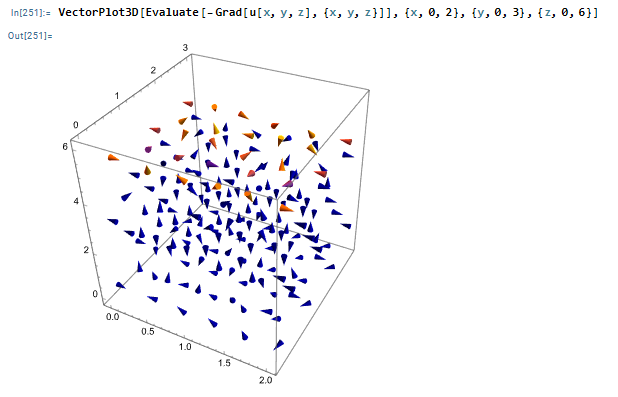
\includegraphics[width=1\linewidth]{image1.png}
\end{figure}
\newpage
\section*{Задача 2}
\subsubsection*{Получение решения}
Перепишем условие задачи:
$$\begin{cases}
    \Delta v=0,\\
    v_x|_{x=0}=v_x|_{x=a}=v|_{y=0}=v_y|_{y=b}=0,\\
    v|_{z=0}=x^3(x-a)^3\sin{(\frac{4\pi y}{24})},\\
    v|_{z=c}=y(y-b)^3\cos{({6\pi x})}.
\end{cases}$$
Проверим выполнение условий согласования:
\begin{enumerate}
    \item $v|_{z=0}=x^3(x-a)^3\sin{(\frac{4\pi y}{24})}:$
    \begin{enumerate}
        \item $(v|_{z=0})_x|_{x=0}=0=(v_x|_{x=0})|_{z=0}, \Rightarrow$ условие выполняется;
        \item $(v|_{z=0})_x|_{x=a}=0=(v_x|_{x=a})|_{z=0}, \Rightarrow$ условие выполняется;
        \item $(v|_{z=0})|_{y=0}=0=(v|_{y=0})|_{z=0}, \Rightarrow$ условие выполняется;
        \item $(v|_{z=0})_y|_{y=b}=0=(v_y|_{y=b})|_{z=0}, \Rightarrow$ условие выполняется.
    \end{enumerate}
    \item $v|_{z=c}=y(y-b)^3\cos{({6\pi x})}:$
    \begin{enumerate}
        \item $(v|_{z=c})_x|_{x=0}=0=(v_x|_{x=0})|_{z=c}, \Rightarrow$ условие выполняется;
        \item $(v|_{z=c})_x|_{x=a}=0=(v_x|_{x=a})|_{z=c}, \Rightarrow$ условие выполняется;
        \item $(v|_{z=c})|_{y=0}=0=(v|_{y=0})|_{z=c}, \Rightarrow$ условие выполняется;
        \item $(v|_{z=c})_y|_{y=b}=0=(v_y|_{y=b})|_{z=c}, \Rightarrow$ условие выполняется.
    \end{enumerate}
\end{enumerate}
Решение этой задачи ищем в виде:
$$v(x,y,z)=X(x)Y(y)Z(z).$$
Подставим в уравнение рассматриваемой задачи и получим:
$$\Delta v=X''YZ+XY''Z+XYZ''=0.$$
Разделим на $XYZ$:
$$\frac{X''}{X}+\frac{Y''}{Y}+\frac{Z''}{Z}=0.$$
$$\frac{X''}{X}+\frac{Y''}{Y}=-\frac{Z''}{Z}=-\lambda^2.$$
$$-\frac{Y''}{Y}-\lambda^2=\frac{X''}{X}=-\mu^2.$$
$$\frac{Y''}{Y}=-\lambda^2+\mu^2=-\nu^2.$$
Рассмотрим две задачи Штурма-Лиувилля для $X(x)$ и $Y(y)$.
$$\begin{cases}
    X''+\mu^2X=0,\\
    X'(0)=0,\\
    X'(a)=0.
\end{cases} \Rightarrow
\begin{cases}
    X(x)=A\cos{\mu x}+B\sin{\mu x},\\
    X'(0)=B=0,\\
    X'(a)=-\mu A\sin{\mu a}=0.
\end{cases}$$
Решением задачи Штурма-Лиувилля для $X(x)$ является:
$$X_n(x)=\cos{(\frac{\pi n}{a}x)},$$
$$\mu_n=\frac{\pi n}{a}, n = 1,2,...$$
Задача для $Y(y)$:
$$\begin{cases}
    Y''+\nu^2Y=0,\\
    Y(0)=0,\\
    Y'(b)=0.
\end{cases} \Rightarrow
\begin{cases}
    Y(y)=A\cos{\nu y}+B\sin{\nu y},\\
    Y(0)=A=0,\\
    Y'(b)=\nu B\cos{\nu b}=0.
\end{cases}$$
Решением задачи Штурма-Лиувилля для $Y(y)$ является:
$$Y_m(y)=\sin{(\frac{\frac{\pi}{2}+\pi m}{b}y)},$$
$$\nu_m=\frac{\frac{\pi}{2}+\pi m}{b}, m = 0,1,...$$
Рассмотрим уравнение для $Z(z)$:
$$\frac{Z_{nm}''}{Z_{nm}}=\lambda_{nm}^2\Rightarrow Z_{nm}''-\lambda_{nm}^2Z_{nm}=0\Rightarrow Z_{nm}=A_{nm}ch(\lambda_{nm}z)+B_{nm}sh(\lambda_{nm}z),$$
где $\lambda_{nm}^2=\mu_n^2+\nu_m^2.$

Таким образом, решение задачи для $v$ представимо в виде:
$$v(x,y,z)=\sum_{n=1}^\infty \sum_{m=0}^\infty(A_{nm}ch(\lambda_{nm}z)+B_{nm}sh(\lambda_{nm}z))\cos{(\frac{\pi n}{a}x)}\sin{(\frac{\frac{\pi}{2}+\pi m}{b}y)}.$$
Для нахождения коэффициентов $A_{nm}$ и $B_{nm}$ воспользуемся граничными условями на $z$.
$$v|_{z=0}=\sum_{n=1}^\infty \sum_{m=0}^\infty A_{nm}\cos{(\frac{\pi n}{a}x)}\sin{((\frac{\pi}{2b}+\frac{\pi m}{b})y)}=x^3(x-a)^3\sin{(\frac{\pi y}{6})}.$$
Отсюда получаем, что $A_{nm}=0,\ \forall m \neq 0,$ а $$A_{n0}=\frac{2}{a}\int_0^a x^3(x-a)^3 \cos(\frac{\pi n}{a}x)dx=[Wolfram\  Mathematica]=-\frac{768 \left(\pi ^2 n^2-60\right) ((-1)^n+1)}{\pi ^6 n^6}.$$ Здесь видно, что при нечетных $n$ $A_{n0}=0,$ тогда получаем, что 
$$A_{n0}=-\frac{1536 \left(4\pi ^2 k^2-60\right)}{64\pi ^6 k^6},\ n=2k.$$
Тогда
$$v|_{z=c}=\sum_{k=1}^\infty (A_{2k0}\ch(\lambda_{2k0}c)+B_{2k0}\sh(\lambda_{2k0} c))\cos(\frac{2\pi k}{a}x)\sin{(\frac{\pi y}{6})}+$$
$$+\sum_{n=1}^\infty \sum_{m=0}^\infty B_{nm}\sh{(\lambda_{nm} c)}\cos{(\frac{\pi n}{a}x)}\sin{(\frac{\frac{\pi}{2}+\pi m}{b}y)}=y(y-b)^3\cos{({6\pi x})}.$$
Отсюда получаем, что $A_{2k0}\ch(\lambda_{2k0}c)+B_{2k0}\sh(\lambda_{2k0} c)=0,$ при $m=0$, то есть $B_{2k0}=-A_{2k0}\cth(\lambda_{2k0}c)\ \forall\ n=2k \neq 12$, а для $n=12$: 
$$B_{12m}=\frac{2}{b}\int_0^by(y-b)^3\sin{(\frac{\frac{\pi}{2}+\pi m}{b}y)}dy=-\frac{96 b^4 \left((2 \pi  m+\pi )^2+2 \pi  (2 m+1)(-1)^m-16\right)}{(2 \pi  m+\pi )^5}.$$
В остальных случаях $B_{nm}=0$.
Таким образом, получаем, что решение исходной задачи принимает вид:
$$v(x,y,z)=\sum_{k=1}^\infty (A_{2k0}\ch(\lambda_{2k0}c)+B_{2k0}\sh(\lambda_{2k0} c))\cos(\frac{2\pi k}{a}x)\sin{(\frac{\pi y}{6})}+$$
$$+\sum_{m=1}^\infty B_{12m}\sh(\lambda_{12m}z)\cos(6\pi x)\sin{(\frac{\frac{\pi}{2}+\pi m}{b}y)}$$

\subsection*{Визуализация решения}
\begin{figure}
    \centering
    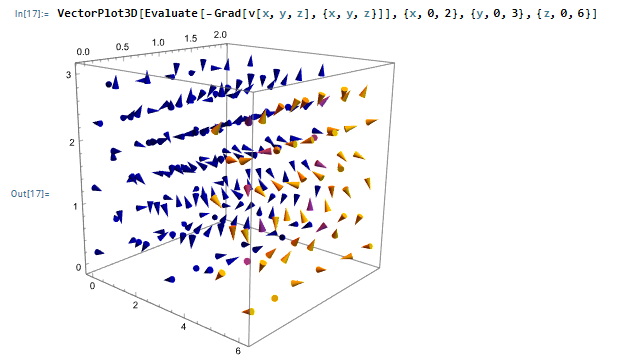
\includegraphics[width=1\linewidth]{image2.png}
\end{figure}
\end{document}
